% Created 2022-02-22 Tue 23:00
% Intended LaTeX compiler: pdflatex
\documentclass[11pt]{article}
\usepackage[utf8]{inputenc}
\usepackage[T1]{fontenc}
\usepackage{graphicx}
\usepackage{longtable}
\usepackage{wrapfig}
\usepackage{rotating}
\usepackage[normalem]{ulem}
\usepackage{amsmath}
\usepackage{amssymb}
\usepackage{capt-of}
\usepackage{hyperref}
\usepackage[margin=0.5in]{geometry}
\author{Marc Soda Jr}
\date{\today}
\title{CSE-343 | Return to Libc Attack Lab}
\hypersetup{
 pdfauthor={Marc Soda Jr},
 pdftitle={CSE-343 | Return to Libc Attack Lab},
 pdfkeywords={},
 pdfsubject={},
 pdfcreator={Emacs 27.2 (Org mode 9.5.2)},
 pdflang={English}}
\begin{document}

\maketitle
\tableofcontents

\section*{Setup:}
\label{sec:org1df65f8}
\begin{itemize}
\item Ran sudo sysctl -w kernel.randomize\textsubscript{va}\textsubscript{space}=0
\item Ran sudo ln -sf /bin/zsh /bin/sh
\item Ran export MYSHELL=/bin/sh
\end{itemize}
\section*{Task 1: Finding the address of libc functions:}
\label{sec:org58ca0e7}
\begin{center}
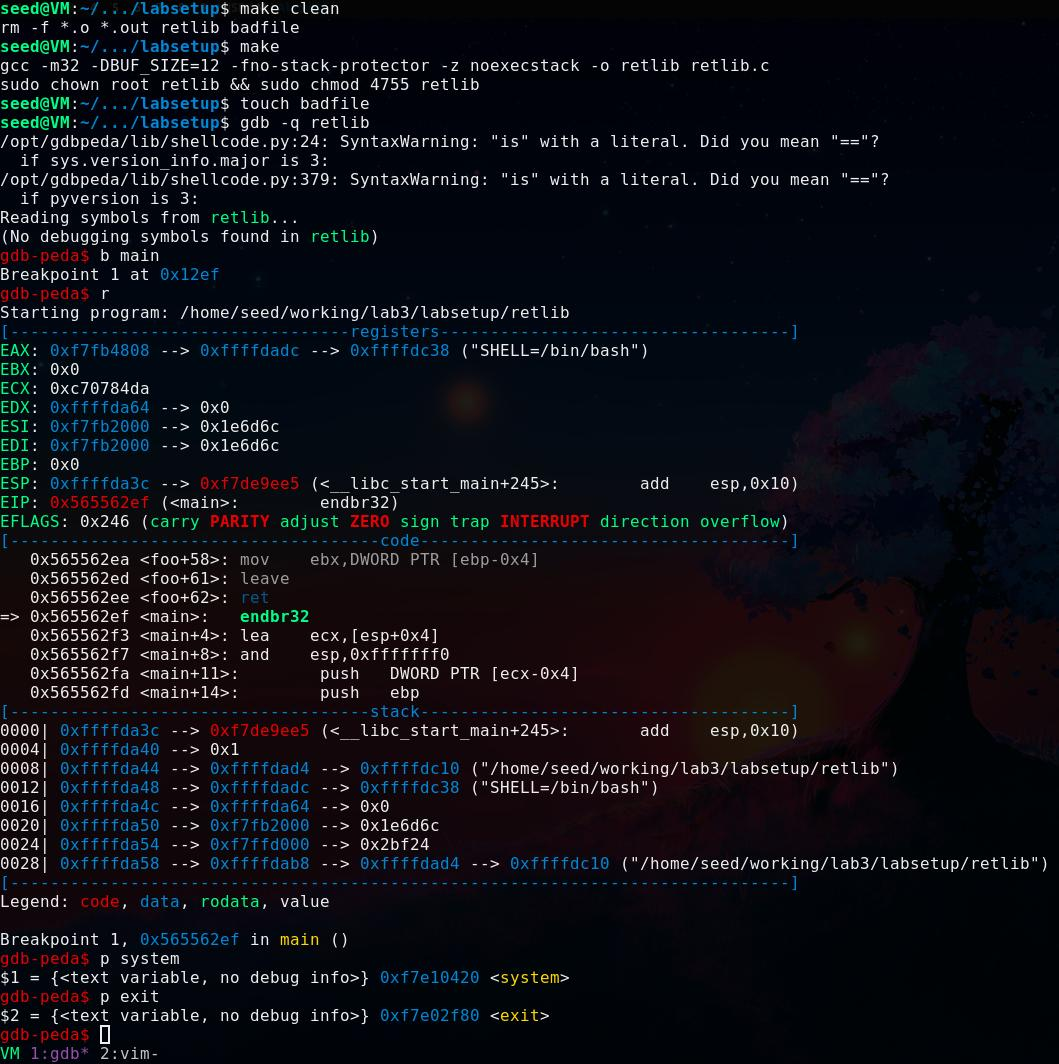
\includegraphics[width=.9\linewidth]{./images/0.jpg}
\end{center}
\begin{itemize}
\item Address of system: 0xf7e10420
\item Address of exit: 0xf7e02f80
\end{itemize}
\section*{Task 2: Putting the shell string in the memory:}
\label{sec:org28df17e}
\begin{center}
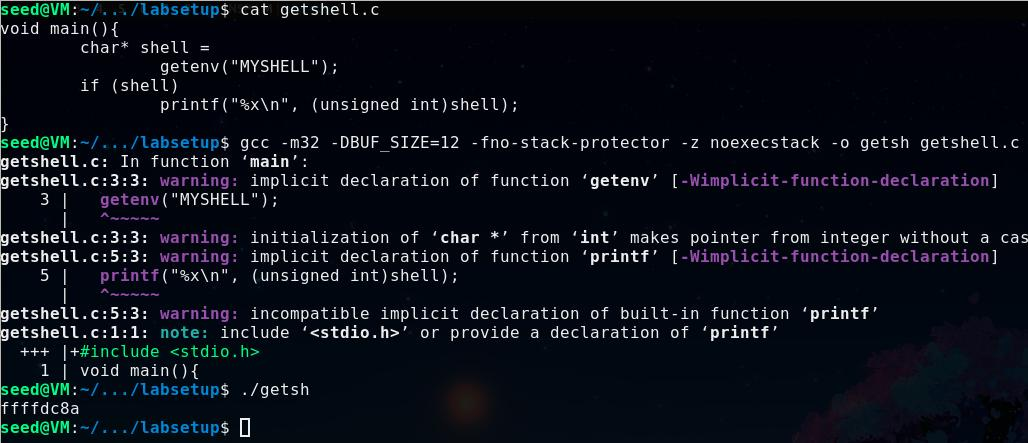
\includegraphics[width=.9\linewidth]{./images/1.jpg}
\end{center}
\begin{itemize}
\item Address of shell: 0xffffdc8a
\item There are, however, some complications with this address that I will hit on later.
\end{itemize}
\section*{Task 3: Launching the attack:}
\label{sec:org2742746}
\begin{itemize}
\item Getting X, Y, and Z.
\begin{center}
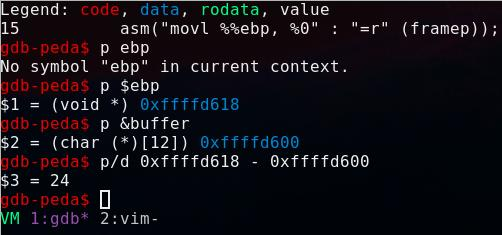
\includegraphics[width=.9\linewidth]{./images/3.jpg}
\end{center}
\begin{itemize}
\item We need to know the distance between ebp and buffer to know the relative location of Y. We know the relative distance between Y and Z (system and exit) is 4 bytes and the relative distance between Z and X (exit and shell) is 4 bytes. As you can see, the distance between ebp and the buffer is 24 bytes which means system starts at 28, exit is at 32, and shell is at 36.
\end{itemize}
\end{itemize}
\begin{center}
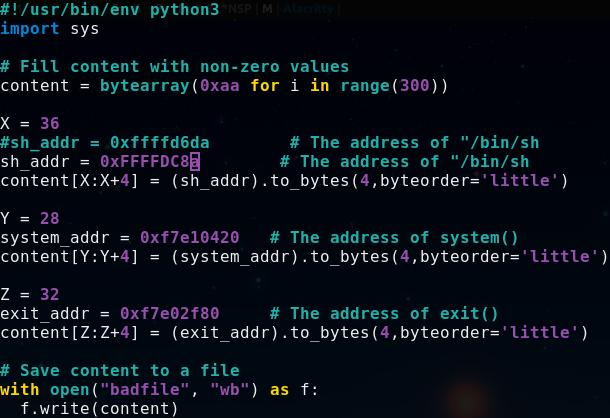
\includegraphics[width=.9\linewidth]{./images/2.jpg}
\end{center}
\begin{itemize}
\item All offsets and memory locations have been filled in the exploit program as stated above, however there is a problem with one of the memory locations:
\end{itemize}
\begin{center}
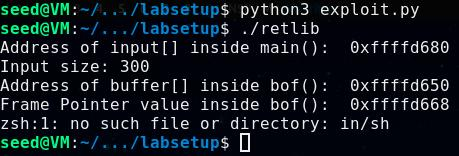
\includegraphics[width=.9\linewidth]{./images/4.jpg}
\end{center}
\begin{itemize}
\item The error messages says that zsh cannot find 'in/sh'. We are trying to hit '/bin/sh' which means we are missing two characters. To solve this issue I subtracted 2 from the shell address (changed 0xffffdc8a to 0xffffdc88). After running it again, we get:
\end{itemize}
\begin{center}
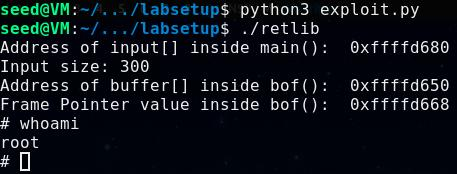
\includegraphics[width=.9\linewidth]{./images/5.jpg}
\end{center}
\begin{itemize}
\item We made it to a root shell. The attack was successful.
\end{itemize}
\section*{Task 4: Defeat Shell's countermeasure.}
\label{sec:orgc43c0b1}
\begin{itemize}
\item Ran 'sudo ln -sf /bin/dash /bin/sh'
\item I edited the provided code for grabbing addresses of env vars to get /bin/bash and -p
\end{itemize}
\begin{center}
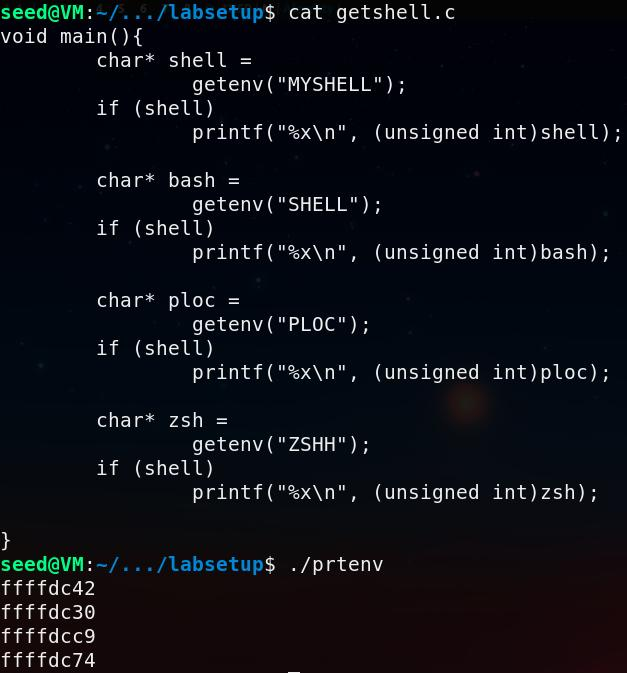
\includegraphics[width=.9\linewidth]{./images/7.jpg}
\end{center}
\begin{center}
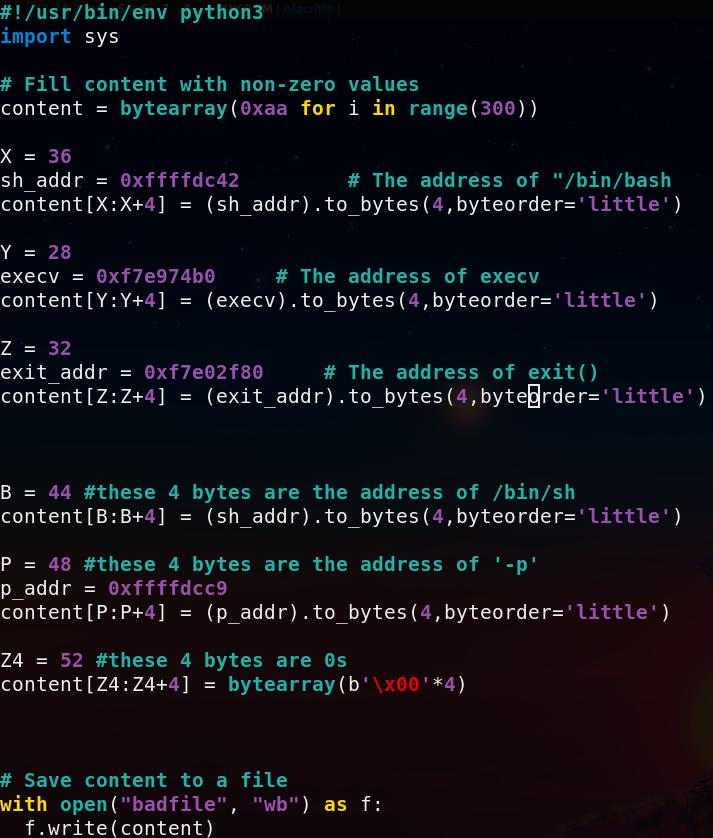
\includegraphics[width=.9\linewidth]{./images/6.jpg}
\end{center}
\begin{itemize}
\item I was unable to get this to work. I am sure I added the addresses in the correct order. I believe my error is in the offset between the first arg of execv and the argv array. I am pretty sure I'm on the right track. My piazza post was not answered in time so I was unable to complete the assignment.
\end{itemize}
\end{document}